\documentclass[12pt, a4paper, twoside]{article}

%% Preamble
\usepackage{pdfpages}           % Para incluir PDFs
\usepackage{graphicx}           % Para gráficos
\usepackage{subfiles}           % Para manejar subarchivos
\usepackage{hyperref}           % Para enlaces
\usepackage{listings}           % Para código fuente (ajusta lenguaje)
\usepackage{verbatim}
\usepackage[backend=bibtex,style=numeric]{biblatex} % Para citas numéricas
\addbibresource{references.bib} % Cargar archivo .bib
\usepackage{url}
\usepackage{float}


\usepackage{geometry}           % Para ajustar márgenes

% Ajustes de márgenes
\geometry{
	left=3cm,       % Margen izquierdo
	right=3cm,      % Margen derecho
	top=2.5cm,      % Margen superior
	bottom=2.5cm,   % Margen inferior
	headheight=15pt, % Altura del encabezado
	twoside          % Para documentos a dos caras
}


\graphicspath{{images/}{../images/}} % Ruta para imágenes

\begin{document}
	
	%% Cover
	
\includepdf[noautoscale=true, width=\paperwidth]{cover.pdf}
	
	%% Title
	\clearpage
	\setcounter{page}{1}
	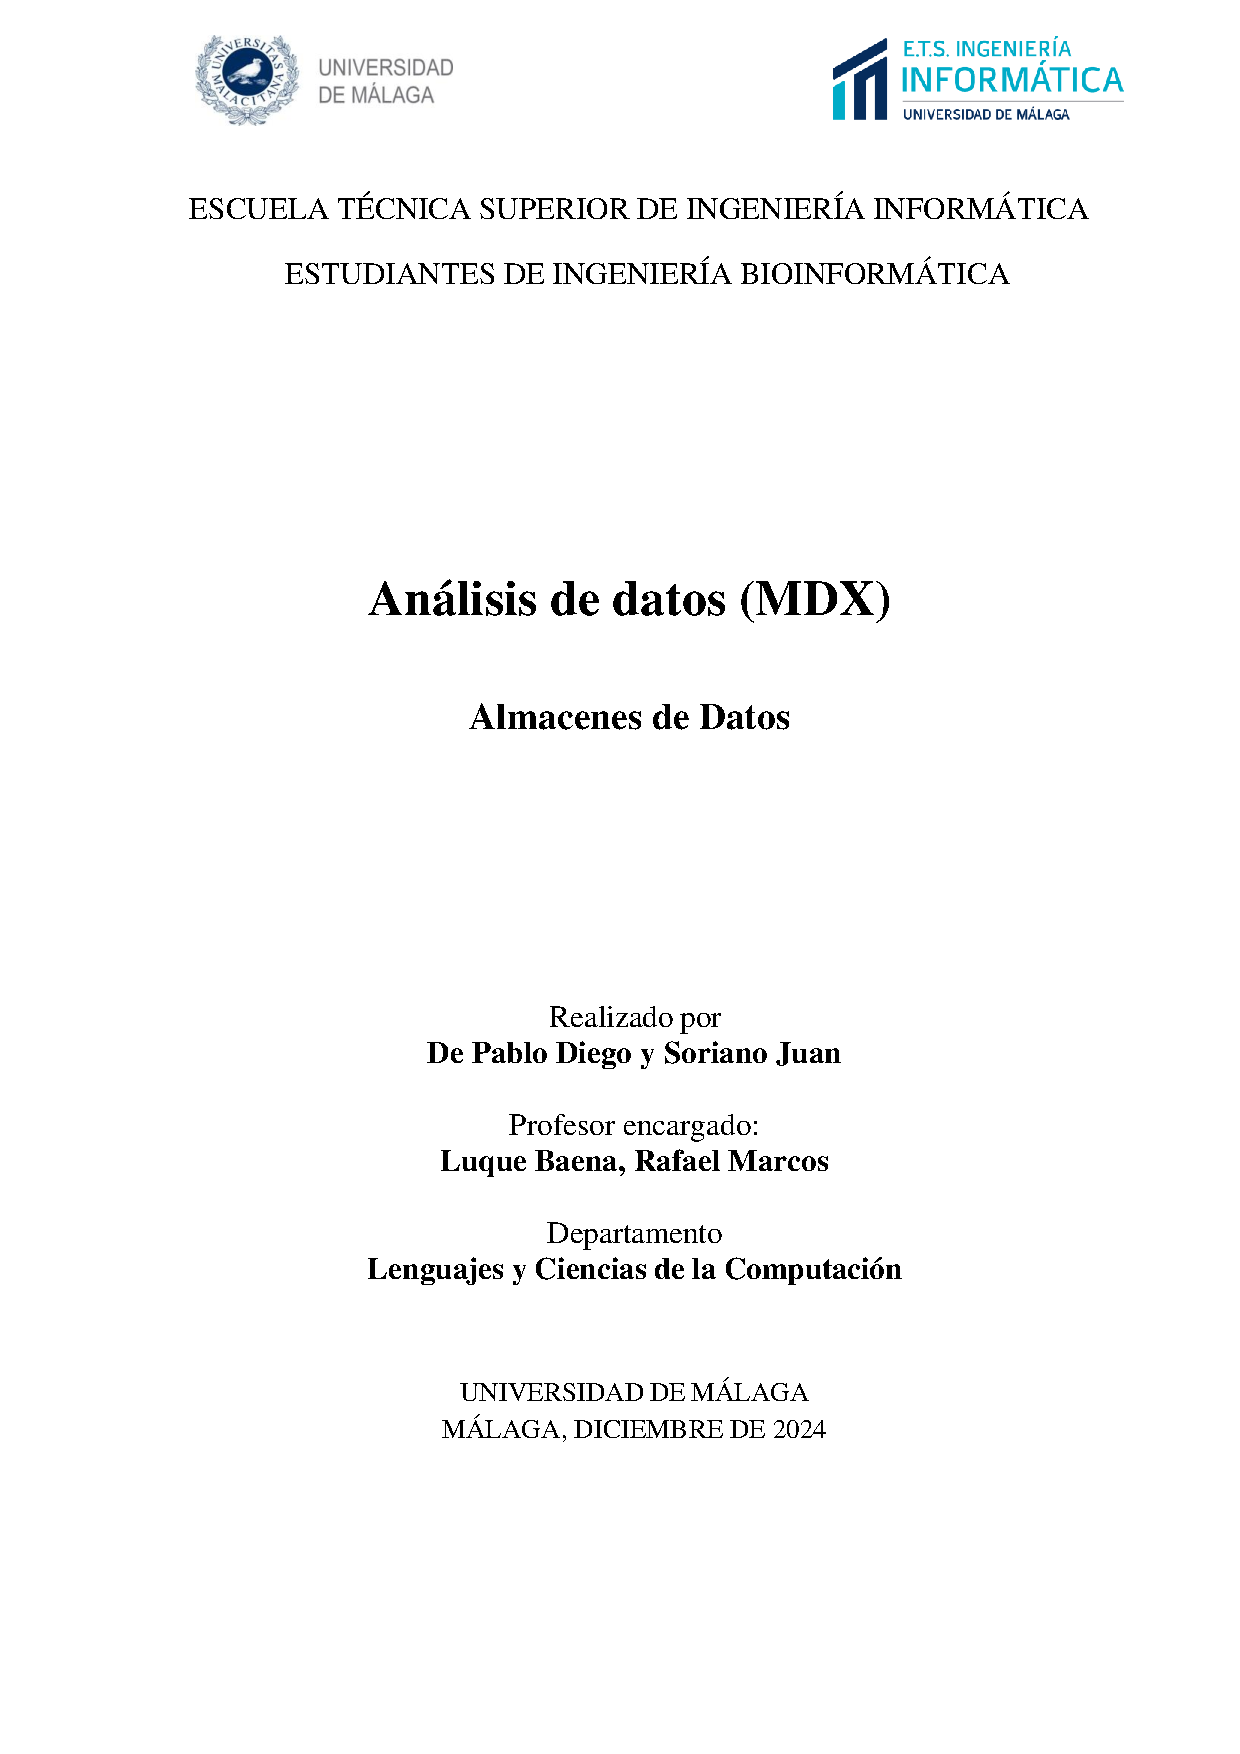
\includepdf[noautoscale=true, width=\paperwidth]{title.pdf}
	
	%%%%%%%%%%%%%%%%%%%%%%%%%%%%%%%%%%%%%%%%%%%%%%%%%%%%%%%%%%%%%%%%%%%%%%%%%%%
	
	% Índice automático
	\tableofcontents
	\newpage
	
	\section{Introducción}
	
	Este documento es una continuación de las fases anteriores del proyecto, donde se desarrollaron el \textbf{diseño conceptual y lógico} de un almacén de datos basado en la información proporcionada por la \textit{Base de Datos de Investigación Colaborativa eICU} \cite{eICU2024}, y la \textbf{integración de datos} mediante un proceso de Extracción, Transformación y Carga (ETL). Para la creación de un almacén enfocado a \textbf{pacientes con patologías respiratorias}.
	
	En esta fase, se busca construir un \textbf{cubo multidimensional} utilizando los datos del almacén previamente desarrollado,	En el ámbito hospitalario, la creación de un cubo multidimensional ofrece ventajas al permitir analizar datos clínicos complejos de manera ágil. Posteriormente se realizarán consultas en \textit{MDX} (Multidimensional Expressions) sobre dicho cubo.  Permitiendo extraer información de manera eficiente al navegar por las dimensiones y medidas del cubo.

	
	Además, se describirán los problemas encontrados durante el desarrollo y las soluciones aplicadas, asegurando que las consultas generen resultados útiles para el análisis de datos.
	
	
	
	\section{Objetivos}
	
	Los objetivos principales de este informe son los siguientes:
	
	\begin{itemize}
		\item Realizar las correcciones pertinentes en el proceso ETL que permitan el desarrollo del cubo muldimensional.
		\item Implementar un cubo multidimensional adaptado para el análisis de \textbf{pacientes con patologías respiratorias}.
		\item Desarrollar al menos 8 consultas en \textit{MDX} que exploren diferentes dimensiones y hechos del cubo, aplicando funciones avanzadas cuando sea necesario.
		\item Documentar de manera clara y replicable el proceso de creación del cubo multidimensional y las consultas \textit{MDX}, proporcionando instrucciones detalladas para su ejecución.
		\item Describir los problemas encontrados durante el desarrollo del cubo y las consultas, y detallar las soluciones empleadas.
	\end{itemize}
	
	
	 
	
	\section{Modificación del almacén de datos}
	
	Eliminamos Age y PatientUnitStayID de paciente
	Cogemos los Pacientes únicos quedándonos con su primera aparición en la base de datos
	Antes nos daba 1849 y ahora después del cambio mencionado en la segunda línea nos salen 1841 como debe ser
	El tiempo seleccionarlo con distinct y diagnosis coger el primer string del DiagnosisString (la primera dimension)
	Corregimos la creación de las tablas intermedias para las relaciones NxM
	
	
	
		- En caso de que se haya tenido que modificar el almacén y el ETL, se ha incluido una sección que indica brevemente las modificaciones realizadas y por qué ha sido necesario acometerlas.
	
	\section{Creación del cubo}
	
	  - Una sección que describa, a modo de tutorial, el proceso para la creación del cubo de vuestro proyecto. 
	  
	  
	  	- La memoria es descriptiva y completa, describiendo correctamente, a modo de tutorial, los pasos para la creación del cubo multidimensional.
	  
	  - Existe un conjunto de instrucciones para desplegar el proyecto en el equipo y es posible su implementación siguiéndolas. 
	
	\section{Consultas en MDX}
	- Una sección con las consultas en MDX y una captura con el resultado de cada una de ellas (la imagen capturada no tiene por qué mostrar todas las tuplas resultantes). 
	
	
	\section{Instrucciones para ejecutar las consultas.}
	- Una sección con las instrucciones detalladas para que un evaluador pueda ejecutar las consultas en su máquina. 
	
	
		- Para cada consulta MDX, se muestra, además del enunciado de la consulta en sí, la consulta realizada en MDX y una captura del resultado generado.
	
	- Indica el número de consultas MDX que se han intentando, es decir, que se ha escrito código MDX y se ha mostrado el resultado de la misma, independientemente de si son correctas o no:
	
	(***) 8 o más.
	
	
	- Según tu experiencia, valora cómo están realizadas las consultas en MDX, seleccionando la opción más adecuada:
	
	(****) Todas las consultas parecen ser correctas, teniendo sentido la salida de cada una de ellas. 
	
	
	- En algunas consultas se han usado funciones más avanzada de MDX, que impliquen el uso de métodos para recorrer una jerarquía (PREVMEMBER, CURRENTMEMBER, PARENT, etc.). 

	\section{Problemas encontrados}


	Maldita maquina virtual




	- Una sección "problemas encontrados" que explique con cierto detalle los problemas que se han encontrado durante la realización de la práctica. Se permite que la información incluida en esta sección se encuentre dividida o dispersada a lo largo del documento. 

	- La sección de "problemas encontrados” (o similar) es coherente y explica con cierto detalle los problemas que se han encontrado durante la realización de la práctica (ojo, no tienen por qué haber sido resueltos). Se permite que la información incluida en esta sección se encuentre dividida o dispersada a lo largo del documento.
	

	- Calificación final.
	

	\section{Conclusión}
	
	XD


	\section{Github y conjunto de instrucciones para su correcto despliegue en SQL Server.}

	Todo el proyecto está accesible en github \cite{depab2024} donde se detalla más específicamente como desplegar en SQL.
	%%%%%%%%%%%%%%%%%%%%%%%%%%%%%%%%%%%%%%%%%%%%%%%%%%%%%%%%%%%%%%%%%%%%%%%%%%%
	\printbibliography
	
	
	%% Back Cover
	
\includepdf[noautoscale=true, width=\paperwidth]{backcover.pdf}
	
\end{document}